\chapter{Discretization Schemes} \index{Discretization schemes|(} \label{cha:discretization_schemes}

\section{Introduction}

Many of the most important and widely used algorithms to study
electromagnetic problems (the \emph{Finite Different Time Domain}, the
\emph{Finite Element}\index{Finite Element method} and the \emph{Finite Volume} methods, to cite
only a few) are based on some sort of discretization of the
four-dimensional space-time domain in which the physical problem is
set \cite{bolla_piers}.

Some of them are based on the differential formulation of Maxwell
equations described in \cite{maxwell_treatise}, others on their
integral formulation \cite{tonti_formulazione}. The former is
independent on the particular reference system in which the equations
are defined: nonetheless, to be able to solve them, one needs to be
set. The latter is not connected to a particular discretization
scheme, but one needs to be defined to be able to solve them.

We can always pass from an integral (or global) representation to a
differential one by a \emph{limiting process}, though. This is how
from experiments, which are integral processes, differential equations
have been induced. While this is very convenient in theory, because
many analytical tools are available for differential equations, it is
not so useful in practice, when Maxwell equations must be solved on a
computer. Its finite nature suggests to avoid this limiting process
\cite{lao_tzu}.

In this chapter, we will focus our attention of the integral
formulation of Maxwell equations and on the discretization process
necessary to solve them. Two steps can be identified:
\begin{enumerate}
\item
  first of all, the three spatial dimensions and the time dimension
  are divided into some ``elementary'' geometrical objects (one-, two-,
  three- and four-dimensional), which,
  altogether, compose a \emph{space-time mesh}, also called \emph{cell
    complex};
\item
  then, if the physical quantities used in the differential
  formulation are functions of points in the four-dimensional domain,
  i.e. functions of points in space and instants in time, in the
  integral formulations they are strictly connected with geometrical
  elements: this association must then be defined.
\end{enumerate}

Many algorithms are available, nowadays. We have studied them, looking
for their best characteristic and trying to condense them into a
unique algorithm.

One source of errors in the Finite Difference Time Domain\index{Finite Difference Time Domain method}
\cite{yee_numerical}, \FDTD for short, for example, is due to the
staircase approximation of metallic boundaries, not parallel to one of
the coordinate planes in the orthogonal grid used
\cite{cangellaris_analysis}. The main effects are:
\begin{itemize}
\item
  numerical dispersion due to the staircase approximation is more
  severe than that for the \FDTD approximation of Maxwell equations
  on an infinite grid;
\item
  non-physical surface modes are supported in the numerical solution by
  the sawtooth conducting boundary;
\item
  waves propagating along the conducting surface are slowed down
  (i.e. the mode of a metallic waveguide with walls parallel to the
  coordinate axis runs faster than one with walls tilted);
\item
  high frequencies suffer more that low frequencies.
\end{itemize}

In \cite{cangellaris_analysis} are reported some solutions to treat
these boundaries. One of them is to use an unstructured grid, instead
of an orthogonal one: this powerful characteristic is included in the
algorithm described in the following sections.

\section{Mesh} \index{Mesh|(}

\subsection{Definition and Properties} \label{sec:mesh:def}

The definition of ``mesh'', also known as ``simplicial
complex''\index{Simplicial complex}, passes
through the definition of ``simplices''.

\begin{definition}[Simplex] \label{def:simplex}
  Given $x_0,x_1,\dotsc,x_M$ affine points in an abstract space, an
  $M$-simplex $\sigma^M$ is the set of points given by:
  \begin{equation*}
    x = \sum_{i=0}^M \lambda_i x_i,
  \end{equation*}
  where $\lambda_i$ are the \emph{barycentric coordinates}\index{Barycentric!coordinates} (see
  \appref{app:barycentric}) such that $\sum_{i=0}^M \lambda_i = 1$ and
  $\lambda_i \ge 0$. We write $\sigma^M = [x_0,x_1,\ldots x_M]$
  \cite{teixeira_geometric}.
\end{definition}

In a three-dimensional space, a $0$-simplex is a point (or vertex or
node or instant in time), a $1$-simplex is a line segment (or edge or
interval in time), a $2$-simplex is a surface (or face, usually a
triangle), and a $3$-simplex is a volume (or cell, usually a
tetrahedron). An \emph{oriented} M-simplex changes sign under a change
of orientation\index{Orientation}, i.e., if $\sigma^M = [x_0,x_1,\dotsc,x_M]$ and a
permutation of the indices is carrier out, then
$[x_{\tau(0)},x_{\tau(1)},\dotsc, x_{\tau(M)}] = (-1)^\tau \sigma^M$,
where $\tau$ denotes the total number of permutations needed to
restore the original index order. The $j$-face of a simplex is the set
defined by $\lambda_j = 0$. The faces of a 1-simplex $[x_0,x_1]$ are
the points $[x_0]$ and $[x_1]$ (0-simplices), the faces of a 2-simplex
$[x_0,x_1,x_2]$ are its three edges $[x_0,x_1]$, $[x_1,x_2]$,
$[x_2,x_0]$ (1-simplices), and so forth.

\begin{definition}[Simplicial Complex]\index{Simplicial complex} \label{def:simplicial_complex}
  A \emph{simplicial complex} $\Set{K}$ is a collection of simplices such
  that:
  \begin{itemize}
  \item
    for all $\sigma^M$ belonging to $\Set{K}$, its faces also belong to
    $\Set{K}$;
  \item
    for any two simplices their intersection is either empty or it is a
    common face of both.
  \end{itemize}
\end{definition}

We note that the concept of simplicial complex is \emph{independent of
  a metric}: this will be a key point in understanding why it is the
general structure over which the discretized version of Maxwell's
equations will be cast.

For a given simplicial complex, let $\Set{N}$ be the set of nodes
$\Point{n}$, $\Set{E}$ the set of edges $\Line{e}$, $\Set{F}$ the set
of faces $\Surface{f}$ and $\Set{V}$ the set of volumes $\Volume{v}$
\cite{trevisan_geometric,rienen_frequency}.

\subsection{Orientation} \index{Orientation|(} \label{sec:mesh:orientation}

In \defref{def:simplex}, an oriented $M$-simplex has been
defined. Moreover, we can define an \emph{oriented mesh} as a normal
mesh, as defined in \defref{def:simplicial_complex}, but with all the
$M$-simplices oriented themselves.

Orientation if very important. While in the differential formulation
of Maxwell equations the physical quantities can be vectors (like
$\E$, $\B$, etc.) defined for each point of the domain, in the
integral formulation equations involve always scalar quantities. This
does not mean that we are losing information associated with the
vectorial nature of quantities in the differential equations: we have
simply switched this information from the physical quantities
themselves to the reference system we are using to represent them. For
example, the vectorial nature of the electric field $\E$ is translated
into the \emph{orientation dependence} of its circuitation along a
line: if the line has an orientation, inverting it means changing the
sign of the circuitation of $\E$ along it.

The are two ways to orient geometrical elements \cite{tonti_formulazione}.
\begin{description}
\item[Internal orientation] We can think of it as an indication of the
  oriented direction \emph{along} the geometrical element: it can be
  defined without the need to ``leave'' the geometrical element
  itself (see \figref{fig:internal_orientation}). A line is internally
  oriented by defining a verse along it, i.e. by
  choosing which are the first and the second nodes of the edge; a
  surface, by internally orienting its boundary in a \emph{coherent}
  way, so that each node on its boundary is the first node of an edge
  and the second of the adjacent edge at the same time; a volume, by
  internally orienting all its boundary faces in a \emph{coherent}
  way, matching the orientation of edges between two adjacent
  faces. Points can be internally oriented too, even if they have null
  measure: the definition can be made indirectly. From points, we can
  trace lines going outward or inward, so defining its orientation:
  conventionally, a point from which all the lines go outward is
  defined a ``source'', or \emph{negatively oriented}; a points from
  which all the lines to inward is defined a ``sink'', or
  \emph{positively oriented}. We call \emph{incidence number} between
  an oriented line and an oriented point the number $+1$ if the
  orientation of the line agrees with the orientation of the point,
  $-1$ otherwise. A typical example is the definition of one
  dimensional increment $\Delta$ of a function $f$ in the interval
  $[x,x+h]$:
  \begin{equation*}
    \Delta f(x) = (-1) f(x) + (+1) f(x+h).
  \end{equation*}
  
  As long as the interval can be internally oriented from its first
  point to the last (it is indeed a one-dimensional vector),
  automatically an internal orientation for its first and second
  points is defined: note that the $+1$ is associated with the point
  $x+h$, which is the sink. Analogously, instants and intervals in
  time can be internally oriented.

  \begin{figure}[htbp]
    \begin{center}
      \subfigure[Point]{\resizebox{4cm}{!}{\input{pics/tonti_fig2_point_inner.pdf_t}}}
      \subfigure[Line]{\resizebox{4cm}{!}{\input{pics/tonti_fig2_line_inner.pdf_t}}}
      \subfigure[Face]{\resizebox{4cm}{!}{\input{pics/tonti_fig2_face_inner.pdf_t}}}
      \subfigure[Volume]{\resizebox{4cm}{!}{\input{pics/tonti_fig2_volume_inner.pdf_t}}}
  \end{center}
    \caption{Internal orientation.}
    \label{fig:internal_orientation}
  \end{figure}
  
\item[External orientation] We can think of it as the oriented
  direction \emph{through} the geometrical element: it can be defined
  only if we suppose to watch the $p$-dimensional geometrical element
  from a $(p+1)$-dimensional point of view (see
  \figref{fig:external_orientation}). For example, a surface
  ($2$-dimensional element) can be externally oriented by
  distinguishing its two faces (and this requires to watch it from a
  $3$-dimensional point of view) and defining a verse through it: in
  other words, an oriented line not lying on the surface can
  externally orient it by distinguishing which of the two faces of the
  surface itself is crossed first. The same can be done with a line,
  which can be externally oriented by defining an internally oriented
  surface not containing the line itself, or a volume, by defining an
  internally oriented point inside it. Even a point can be
  externally oriented, by defining an internally oriented volume
  containing it. Again, the same is applicable to instants and
  intervals in time.

  Note that internally oriented $p$-dimensional elements are used to externally orient
  $(3-p)$-dimensional elements: this will be used in the orientation
  of the dual mesh (\secref{sec:dual_mesh}).
  
  A word about notation: externally oriented geometrical elements can
  be distinguished by the internally oriented for the tilde on top. So:
  $\ExtOrient{\Point{p}}$, $\ExtOrient{\Line{e}}$, $\ExtOrient{\Surface{f}}$ and
  $\ExtOrient{\Volume{v}}$ are externally oriented point, edge, face and
  volume, respectively.

  \begin{figure}[htbp]
    \begin{center}
      \subfigure[Point]{\resizebox{4cm}{!}{\input{pics/tonti_fig2_point_outer.pdf_t}}}
      \subfigure[Line]{\resizebox{4cm}{!}{\input{pics/tonti_fig2_line_outer.pdf_t}}}
      \subfigure[Face]{\resizebox{4cm}{!}{\input{pics/tonti_fig2_face_outer.pdf_t}}}
      \subfigure[Volume]{\resizebox{4cm}{!}{\input{pics/tonti_fig2_volume_outer.pdf_t}}}
  \end{center}
    \caption{External orientation.}
    \label{fig:external_orientation}
  \end{figure}

\end{description}

An example to distinguish between internal and external orientation can be
made thinking about inversion of time. There are physical quantities
which are left unchanged by an inversion of time (like the total
electric charge inside a volume) and others that change their sign
(like the electric charge that pass through a given surface). The
first ones are associated with internally oriented instants or
externally oriented intervals and the seconds with externally oriented
instants or internally oriented intervals \cite{tonti_formulazione}.

Given the domain to discretize, the choice of the simplicial cell
complex is not unique. One very common way of defining a cell complex
is by triangles in two dimensions or tetrahedral in three
dimensions. These are the easiest geometrical shapes that satisfy the
properties in \defref{def:simplicial_complex} and they are therefore
called \emph{simplicial elements}: each more complicated shape
(squares, polygons, parallelepipeds, \ldots) can be simplified into
simplicial elements. Moreover, very often, simplicial elements which
satisfy another property are used to build simplicial complexes, which
are called \emph{Delaunay simplicial complexes}\index{Delaunay}. Their peculiar
property is that each circumcenter (or circumsphere in three
dimensions) associated to a cell does not contain any other vertices
apart from the ones that define the cell itself. This property has a
very important consequence on the stability of the algorithms
associated with this mesh. Consider, for example,
\figref{fig:tonti_thermal}: a thermal field is defined on the cells
$t_1$ and $t_2$, and $T_1 > T_2$ are the
temperatures measured at points $C_1$ and $C_2$, respectively. Heat
flows naturally from the warmer zone to the colder, through the common face
between cells $t_1$ and $t_2$. But if the verse of the segment
$C_1C_2$ is opposed to the verse of the segment going from $t_1$ to
$t_2$, the heat flux will be negative (i.e., in the opposite
direction, from a colder zone to a warmer zone), which is
non-physical. This process is going to increase without limit: it's an
instability\index{Instability} \cite{tonti_formulazione}. This is due to the fact that
the mesh in \figref{fig:tonti_thermal:bad} is not a Delaunay mesh.

Something very similar can happen in electromagnetic simulations with
fluxes and circuitations of vectorial fields.

\begin{figure}[htbp]
  \begin{center}
    \subfigure[Delaunay primal mesh.]{\resizebox{!}{5cm}{\input{pics/tonti_thermal.pdf_t}}}
    \subfigure[Non-Delaunay primal mesh.]{\resizebox{!}{5cm}{\label{fig:tonti_thermal:bad}\input{pics/tonti_thermal_bad.pdf_t}}}
  \end{center}
  \caption{The simplicial complex choice affects the stability of
    the algorithm. If a thermal field is defined on the
    triangles $t_1$ and $t_2$ and the temperatures measured at
    points $C_1$ and $C_2$ are $T_1 > T_2$, a thermal flux from the
    colder cell to the warmer will be simulated in the
    right-hand side mesh: this is non-physical.}
  \label{fig:tonti_thermal}
\end{figure}

Another very common three-dimensional mesh is the two-dimensional
extruded mesh: see \figref{fig:extruded_mesh} for an example. It is
made of a two-dimensional mesh, extruded in the third dimension, like
a stack of two-dimensional meshes. The advantage is that simple
two-dimensional meshing software \cite{meshing_software} can be used
to model each ``floor'' of the stack and then it can be very easily
extruded in the third dimension like a structured mesh. Two-dimensional
extruded grids are best suited to model planar geometries: they will
be used to study planar photonic crystal channels (see
\secref{sec:frequency_domain:3D}).

\begin{figure}[htbp]
  \begin{center}
    \resizebox{5cm}{!}{\input{pics/extruded_mesh.pdf_t}}
  \end{center}
  \caption{Two-dimensional extruded mesh. Two-dimensional meshes are
    the ``floors'' of a three-dimensional stack. Distance between
    two-dimensional meshes has been exaggerated, for the sake of
    clarity.}    
  \label{fig:extruded_mesh}
\end{figure}

\index{Orientation|)}

\subsection{Dual Mesh} \label{sec:dual_mesh}

Once we have defined a cell complex $\Set{K}$, orienting its geometrical
elements suggests the definition of another cell complex:
\begin{equation*}
  \Dual{\Set{K}} = \left\{\Dual{\Set{N}}, \Dual{\Set{E}},
  \Dual{\Set{F}}, \Dual{\Set{V}}\right\},
\end{equation*}
made of
points $\Dual{n} \in \Dual{\Set{N}}$, lines $\Dual{e} \in
\Dual{\Set{E}}$, surfaces $\Dual{f} \in \Dual{\Set{F}}$ and volumes
$\Dual{v} \in \Dual{\Set{V}}$ used to externally orient its volumes,
surfaces, lines and points, respectively. This \emph{induced} cell
complex is called \emph{dual} cell complex, and the original one is
called \emph{primal} cell complex \cite{tonti_formulazione}. Some
observations can be made:
\begin{itemize}
\item
  for each cell complex, a dual cell complex can be defined;
\item
  there is a surprising ``symmetrical'' property, for which a vertex
  in a primal cell complex corresponds to a cell in the dual complex, a
  line to a surface, a surface to a line and a volume to a point, an
  instant to an interval and an interval to an instant: an upside-down
  classification of geometrical elements, as shown by the
  \diaref{dia:dual_mesh_symmetry};  

  \begin{equation} \label{dia:dual_mesh_symmetry}
    \begin{CD}
      \Point{n}   @>>> \ExtOrient{\Volume{v}} \\
      @VVV             @VVV \\
      \Line{e}    @>>> \ExtOrient{\Surface{f}} \\
      @VVV             @VVV \\
      \Surface{f} @>>> \ExtOrient{\Line{e}} \\
      @VVV             @VVV \\
      \Volume{v}  @>>> \ExtOrient{\Point{n}} \\
    \end{CD}
  \end{equation}
  
\item
  the choice of the dual mesh is somehow arbitrary: there is no special
  need to choice one particular orientation over another possible
  orientation (even if, conventionally, we use the \emph{pit}'s convention
  for points and volumes and the \emph{right-hand} convention for
  lines and surfaces) or to choose a particular point or line to
  externally orient a volume or a surface of the primal cell
  complex. As we'll see later, though, some choices are better than
  others, therefore some dual meshes are better than others, for
  stability and ease of equations formulation.
\end{itemize}

As said before, the choice of the primal cell complex is not unique:
neither is the choice of its dual. For primal cell complexes, Delaunay\index{Delaunay}
tessellations satisfy some very important properties that have
positive drawbacks on the algorithms'
stability \cite{cavendish_complementary}. Their dual complexes are
called \emph{Vorono\"i}\index{Vorono\"i} complexes and they are defined by taking the
circumcenters (or circumspheres in three-dimensions) of the primal
cells as nodes. Each dual edge will be orthogonal to a primal face and
each dual face will be orthogonal to a primal edge, for
construction. At the limit of very small cells, the couple
Delaunay-Vorono\"i complexes are locally an orthogonal reference
system. As we'll in \secref{sec:voronoi}, this greatly simplifies the
numerical discretization of Maxwell equations.

Another possible choice is to consider the barycenters of primal cells
as the nodes of the dual meshes: it they are connected by straight
lines, the dual edges, the resulting dual mesh is called
\emph{Poincar\'e}\index{Poincar\'e} dual mesh. If, on the other hand, dual edges are
piece-lines going from the barycenter of a primal cell to the
barycenter of an adjacent primal cell passing by the barycenter of the
common primal face, the resulting dual mesh is called
\emph{barycentric}.

\subsection{Matricial Representation} \label{sec:mesh:matricial}

A mesh can be seen as graph, possibly oriented, with edges representing
``relations'' between the nodes. Therefore, many techniques applicable
to graphs can be applied to meshes, as well.

In particular, to represent an oriented mesh \emph{incidence matrices}
can be used. Incidence matrices are matrices (usually sparse) made of
$0$s, $1$s and $-1$s to describe the interconnections between
geometrical elements. If two elements $i$, $j$ are not connected the
matrix element $(i,j)$ is $0$, otherwise it's $\pm 1$: the sign
is positive if the orientation of $i$ agrees with the orientation of
$j$, otherwise is negative.

Mutual interconnections of the simplices in the primal mesh $\Set{K}$
can be described by incidence matrices \cite{trevisan_geometric}:
\begin{itemize}
\item
  $\Matrix{G}$ is the incidence matrix between edges $\Line{e}$ and
  nodes $\Point{n}$;  
\item
  $\Matrix{R}$ is the incidence matrix between faces $\Surface{f}$ and
  edges $\Line{e}$;  
\item
  $\Matrix{D}$ is the incidence matrix between volumes $\Volume{v}$
  and faces $\Surface{f}$.  
\end{itemize}

\begin{figure}[htbp]
  \begin{center}
    \resizebox{4cm}{!}{\input{pics/adiacency_e_n.pdf_t}}
  \end{center}
  \caption{Adjacency edges-nodes. Orientation of edges is shown by the
    arrow sign, while orientation of nodes is conventionally chosen to
    be positive for sinks and negative for sources.}
  \label{fig:adiacency_e_n}
\end{figure}

With respect to figure \ref{fig:adiacency_e_n}, the $k$-row of the matrix
$\Matrix{G}$, incidence matrix between edges and nodes, is:
\begin{align*}
  \Matrix{G} & = \begin{bmatrix}
    \dots & \dots & \dots  & \dots & \dots & \dots & \dots \\
    0     & \dots & -1     & \dots & 1     & \dots & 0     \\
    \dots & \dots & \dots  & \dots & \dots & \dots & \dots
  \end{bmatrix} \leftarrow \text{\color[rgb]{0,0,1}$k$ row} \\
  & \quad \begin{matrix}
    \qquad & \qquad & \mspace{-14mu}\uparrow       & \qquad & \mspace{-28mu}\uparrow       \\
    \qquad & \qquad & \mspace{-14mu}\text{$i$ col} & \qquad & \mspace{-28mu}\text{$j$ col}
  \end{matrix}
\end{align*}
where the $+1$ says that the edge $k$ is entering the node $j$,
i.e. agrees with the ``sink'' convention for oriented nodes.

Something very similar can be done to build the other matrices.

\begin{figure}[htbp]
  \begin{center}
    \resizebox{4cm}{!}{\input{pics/adiacency_f_e.pdf_t}}
  \end{center}
  \caption{Adjacency faces-edges. Orientation of edges is shown by the
    arrow sign, while faces are internally oriented by the curved
    arrow. In the picture, the orientation of the edge $i$ agrees with
    the orientation of the face $l$, while edges $j$ and $k$ have
    opposite orientations.}
  \label{fig:adiacency_f_e}
\end{figure}

With respect to figure \ref{fig:adiacency_f_e}, the $l$-row of the
matrix $\Matrix{R}$, incidence matrix between faces and edges, is:
\begin{align*}
  \Matrix{R} & = \begin{bmatrix}
    \dots & \dots & \dots  & \dots & \dots & \dots & \dots & \dots    & \dots \\
    0     & \dots & 1      & \dots & -1    & \dots & -1    & \dots    & 0     \\
    \dots & \dots & \dots  & \dots & \dots & \dots & \dots & \dots    & \dots
  \end{bmatrix} \leftarrow \text{\color[rgb]{0,0,1}$l$ row} \\
  & \quad \begin{matrix}
    \qquad & \qquad & \mspace{-14mu}\uparrow       & \qquad & \mspace{-28mu}\uparrow       & \qquad & \mspace{-28mu}\uparrow \\
    \qquad & \qquad & \mspace{-14mu}\text{$i$ col} & \qquad & \mspace{-28mu}\text{$j$ col} & \qquad & \mspace{-28mu}\text{$k$ col}
  \end{matrix}
\end{align*}
where the $+1$ says that the edge $i$ agrees with the orientation of
the face $l$.

\begin{figure}[htbp]
  \begin{center}
    \resizebox{4cm}{!}{\input{pics/adiacency_v_f.pdf_t}}
  \end{center}
  \caption{Adjacency volumes-faces. Internal orientation of faces is
    shown the curved arrow. The volume is conventionally oriented from
    inside to outside. In the picture, the orientation of the face $i$
    agrees with the orientation of the volume $m$, while the other faces
    disagree.}
  \label{fig:adiacency_v_f}
\end{figure}

Finally, from figure \ref{fig:adiacency_v_f}, the $m$-row of matrix
$\Matrix{D}$, incidence matrix between volumes and faces, is:
\begin{align*}
  \Matrix{D} & = \begin{bmatrix}
    \dots & \dots & \dots  & \dots & \dots & \dots & \dots & \dots & \dots    & \dots \\
    0     & \dots & 1      & \dots & -1    & \dots & -1    & -1    & \dots    & 0     \\
    \dots & \dots & \dots  & \dots & \dots & \dots & \dots & \dots & \dots    & \dots
  \end{bmatrix} \leftarrow \text{\color[rgb]{0,0,1}$m$ row} \\
  & \quad \begin{matrix}
    \qquad & \qquad & \mspace{-14mu}\uparrow       & \qquad & \mspace{-28mu}\uparrow       & \qquad & \mspace{-28mu}\uparrow       & \mspace{-14mu}\uparrow \\
    \qquad & \qquad & \mspace{-14mu}\text{$i$ col} & \qquad & \mspace{-28mu}\text{$j$ col} & \qquad & \mspace{-28mu}\text{$k$ col} & \mspace{-14mu}\text{$l$ col}
  \end{matrix}
\end{align*}
where the $+1$ says that the face $i$ agrees with the orientation of
the volume $m$.

Note also that for a non-pathological meshes:
\begin{align*}
  \nn = \ndv && \ne = \ndf && \nf = \nde && \nv = \ndn \\
  \ndn = \nv && \nde = \nf && \ndf = \ne && \ndv = \nn
\end{align*}
where $n_x$ denotes the number of geometrical elements $x$.

Therefore, we have:
\begin{align*}
  \Matrix{D} & \in \CrossProd{\nv}{\nf} \\
  \Matrix{R} & \in \CrossProd{\nf}{\ne} \\
  \Matrix{G} & \in \CrossProd{\ne}{\nn}
\intertext{and}
   \Transpose{\Matrix{D}} & \in \CrossProd{\nde}{\ndn} \equiv \Dual{\Matrix{G}} \\
   \Transpose{\Matrix{R}} & \in \CrossProd{\ndf}{\nde} \equiv \Dual{\Matrix{R}} \\
  -\Transpose{\Matrix{G}} & \in \CrossProd{\ndv}{\ndf} \equiv \Dual{\Matrix{D}}.
\end{align*}

The matrices $\Transpose{\Matrix{D}}$, $\Transpose{\Matrix{R}}$ and
$-\Transpose{\Matrix{G}}$\footnote{The minus sign comes from the
  assumption that $\Point{n}$ is oriented as a sink, whereas the boundary of
  $\DualVolume{v}$ is oriented by the outer normal.} describe the
interconnections of $\Dual{\Set{K}}$.

\index{Mesh|)}

\section{Geometry and Physics} \label{sec:geometry_and_physics}

There are different discretization schemes for Maxwell
equations. Considering the discretization in time, we can distinguish
two big families of discretization schemes \cite{bolla_piers}:
\begin{description}
\item[collocated schemes], in which physical quantities are all
  associated to the same time. In other words, the discretization
  in time does not depend on the specific physical quantity we are
  modeling;
\item[uncollocated schemes], in which different physical quantities
  are associated with different points in time, as if there were
  different discretization schemes in time for each physical quantity.
\end{description}

The same concept may be applied to the discretization in space, with
the added complexity that the domain to discretize is now three-dimensional,
instead of one-dimensional. The most clearly visible difference is
that the geometrical objects we can use to discretize the space and to
which associate the physical quantities can be points, lines, surfaces
or volumes: much more freedom than in time, where we just have points
(instants) and lines (intervals)!

Again, we can distinguish \cite{bolla_piers}:
\begin{description}
\item[unstaggered schemes]: they are analogous to collocated
  schemes in time, in the sense that physical quantities are all
  associated to the geometrical elements of a unique mesh;
\item[staggered schemes]: in which each physical quantity has its
  own discretization in space. These are the analogous of
  uncollocated schemes in time.
\end{description}

Until now, we have spoken of ``associating physical quantities to
geometrical elements'': with this expression, we intend to create a
map between physical quantities, such as fields, potentials or
charges, and geometrical elements, such as points, lines, faces and
volumes. The result of the map will be a scalar, used in the integral
form of Maxwell equations.

Let's start from the integral form of the Maxwell equations:
\begin{equation} \label{eqn:maxwell_integral} \begin{cases}
    \int_{\partial \Surface{S}}{\DotProd{\E}{\d \Vector{l}}} =
    -\partial_t \iint_{\Surface{S}}{\DotProd{\B}{\Versor{n}} \d S} \\
    \int_{\partial \DualSurface{S}}{\DotProd{\H}{\d \Vector{\Dual{l}}}} =
    \partial_t \iint_{\DualSurface{S}}{\DotProd{\D}{\Versor{\Dual{n}}} \d \Dual{S}} \\
\end{cases}, \end{equation}
where, $\partial \Surface{S}$ denotes the boundary of a surface
$\Surface{S}$, $\d \Vector{l}$ a vector tangent to it and $\Versor{n}$
a versor orthogonal to $\Surface{S}$: similar meanings hold for the tilded
variables.

We can distinguish two kinds of physical quantities in
\eqref{eqn:maxwell_integral}. The first equation in
\eqref{eqn:maxwell_integral}, the \emph{Faraday equation}, reads:
``given an oriented surface $\Surface{S}$, the circuitation of the
electric field along its boundary equals the opposite of the
derivative in time of the flux of the magnetic vector through
it''. The second of \eqref{eqn:maxwell_integral}, the \emph{Amp\`ere
law}, reads: ``given an oriented surface $\Surface{S}$, the
circuitation of the magnetic induction equals the derivative in time
of the electric induction plus the flux of the current density through
it''. Many observations can be made:
\begin{itemize}
\item
  Maxwell equations, in the integral form, only relate circuitations
  to fluxes;
\item
  each equation relate a vector ($\E$ or $\D$) with a covector ($\H$
  or $\B$): the curl operator transforms a vector to a covector
  \cite{bossavit_computational};
\item
  the two equations are only topological relations, in the sense that
  they depend only on the topological properties of surfaces and boundaries
  and not on the physical properties of the underlying medium;
  materials link vectors to covectors by material equations: $\D =
  \epsilon \E$ and $\B = \mu \H$;
\item
  we need an oriented space to make the equation work: the orientation
  is arbitrary, but it needs to be coherent;
\item
  in the first equation, if the electric field is evaluated at some
  time $t$, so must be the partial derivative in time of $\B$: the
  same holds for the second equation with $\H$ and $\D$. This will drive
  the choice of a uncollocated discretization scheme in time.
\end{itemize}

The most spontaneous way for the association of physical quantities to
geometrical elements is ``circuitations with
lines'' and ``fluxes with surfaces'': there is no circuitation without
a line and no flux without a surface. We can then define the maps:
\begin{equation} \label{eqn:dof} \begin{aligned}
  \text{primary edge $\Line{e}$} && \Map{e} && \int_{\Line{e}}{\DotProd{\E}{\d\Vector{l}}} \\
  \text{primary surface $\Surface{f}$} && \Map{b} && \iint_{\Surface{f}}{\DotProd{\B}{\Versor{n}}\d S} \\
  \text{primary surface $\Surface{f}$} && \Map{m} && \iint_{\Surface{f}}{\DotProd{\M}{\Versor{n}}\d S} \\
  \text{dual line $\DualLine{e}$} && \Map{h} && \int_{\DualLine{e}}{\DotProd{\H}{\d\Vector{\Dual{l}}}} \\
  \text{dual surface $\DualSurface{f}$} && \Map{d} && \iint_{\DualSurface{f}}{\DotProd{\D}{\Versor{n}}\d\tilde{S}} \\
  \text{dual surface $\DualSurface{f}$} && \Map{j} && \iint_{\DualSurface{f}}{\DotProd{\J}{\Versor{n}}\d\tilde{S}}
\end{aligned} \end{equation}

Maxwell equations are topological relations: as long as
the mesh satisfies the properties in \defref{def:simplicial_complex},
with the association in \eqref{eqn:dof}, they can be written to be
\emph{strictly exact}. So, where are the necessary approximations,
always connected to a discretization process? Obviously, they are
outside Maxwell equations, in particular in the material equations (see
\secref{cha:material_equations})\footnote{It's worth noting that this
  is not the only possibility: some discretization schemes introduce
  errors in Maxwell equations, but model exactly material
  equations. We think that these schemes should not be used because
  they fail to satisfy identically all the properties encoded in
  Maxwell equation, like flux conservation, for example. We think that
  modeling the wrong material is better than modeling the wrong
  physical equations.}.

One might argue, why should we care about dividing metric independent,
i.e. Maxwell, and metric dependent, i.e. material, equations? There
are at least three good answers \cite{teixeira_geometric}:
\begin{enumerate}
\item
  many theorems (such as charge conservation, Faraday equation and
  Amp\`ere law) are automatically fulfilled after discretization,
  without the need to involve metric concepts, because they only
  depend on topology;
\item
  the metric is completely encoded into the material equations, the
  treatment of curved boundaries and material interfaces can be done
  in a more systematic manner, without affecting, for example,
  conservation laws related to the topological equations;
\item
  the topological (spatial) part of the equations often comprises
  integer arithmetic only and are more efficiently handled by a
  computer if, a priori, recognized as such.
\end{enumerate}

\diaref{dia:relations} shows graphically the relations between the
four vectorial fields used in \eqref{eqn:maxwell_integral}.

\begin{equation} \label{dia:relations}
  \begin{CD}
    \E @>{\text{Faraday}}>> \B \\
    @A{\epsilon}AA @VV{\mu}V \\
    \D @<<{\text{Amp\`ere}}< \H
  \end{CD}
\end{equation}

Discretization in time, discretization in space and association of
physical quantities with geometrical elements are ``decoupled''
choices: one particular choice in one, does not limit the choices in
the others. This is the reason why there are so many algorithms, more
or less similar to each others, based on the same concepts of
discretization of Maxwell equations, each sharing the same strengths
and weaknesses. An example of an algorithm based on an uncollocated
staggered scheme is the \emph{Finite Difference Time Domain} method\index{Finite Difference Time Domain method}
\cite{taflove_computational}, in the \emph{Yee
implementation}\cite{yee_numerical}. The same algorithm, but
implemented using the \emph{forward/backward differences} both in time
and in space, becomes a collocated unstaggered scheme
\cite{lavrinenko_comprehensive}. In the frequency domain, where time
doesn't need to be discretized because not present in Maxwell
equations, we can list the \emph{Finite Element}\index{Finite Element method} method, with the node
element base \cite{jin_finite}, as a staggered scheme, or the
\emph{Finite Element} method with the Whitney elements discretization
scheme \cite{bossavit_yee}, as an unstaggered scheme.

Not all the discretization schemes are equally suited to model
electromagnetic problems, though. The geometrical properties of the
physical problem suggest somehow the best discretization scheme to
use, which is also the most elegant \cite{maxwell_mathematical}.

Maxwell equations are two coupled first order partial differential
equations: partial derivatives in space of the electric field are
related to partial derivative in time of the magnetic field and
viceversa. This ``chiasmo'' in space and time strongly suggests to use
an uncollocated staggered scheme, which geometrically suggests the
spatial and temporal interconnection of fields. Indeed, this is the
best choice, leading to simple equation and, more importantly, to the
satisfaction of the equation $\Div{\B} = 0$ everywhere (and every
when) on the grid. The divergenceless of the magnetic field is a
fundamental physical property: any mathematical model deviating from
this fact is incorrect\footnote{As far as modern physics knows
\cite{mead_collective}.} and can lead to instabilities that are
non-physical. \emph{Finite Volume} methods, for example, undergo
non-physical attenuation of waves, for the choice of a collocated
unstaggered scheme \cite{taflove_advances}: it is as if the
discretized medium itself, where the electromagnetic waves are
propagated, were lossy. Losses come from the numerical world, not from
the ``real'' one, though. Collocated scheme are also badly suited to
study coupled equations: they naturally lead to uncoupled equations,
and the coupling, present in Maxwell's equations, is obtained in these
methods only at the expense of elegance in the formalism.

\subsection{Matricial Representation}

In \secref{sec:mesh:matricial}, the incidence matrices of the primal
and dual simplicial complexes $\Set{K}$ and $\Dual{\Set{K}}$ have been
defined, from a purely topological point of view. With the map defined
in \eqref{eqn:dof}, applied to Maxwell equations, they can be seen
under another light \cite{trevisan_geometric}.

$\Matrix{R}$ and $\Dual{\Matrix{R}}$ are the
\emph{discrete curl operators} on the primal and dual grid,
respectively, $\Matrix{D}$ and $\Dual{\Matrix{D}}$ are the
\emph{discrete divergence operators} and $\Matrix{G}$ and
$\Dual{\Matrix{G}}$ are the \emph{discrete gradient
operators}\footnote{This symmetry is better explained with a drawing
  in \appref{app:maxwell_house}.}.

We can grasp a geometrical explanation of these discrete operators
thinking that to compute the divergence of a vectorial field we need to
define a closed surface, on which the field is defined, and make it
smaller and smaller (zero, at limit): the flux through this
infinitesimal surface is the divergence at the point that it
contains. This is the Gauss theorem. In other words, the divergence
is an operator that takes a field defined on a surface and gives a
field defined in a volume (infinitesimally small -- a point): in the
discrete world, it is an operator between a flux through a surface and
a volume integral. In matrix form, it must be a $\CrossProd{\nf}{\nv}$
matrix, like the matrix $\Matrix{D}$. A similar
reasoning holds for the gradient, i.e. the matrix $\Matrix{G}$, and the curl,
i.e. the matrix $\Matrix{R}$. The \diaref{dia:discrete_operators}
shows these relations.

\begin{equation} \label{dia:discrete_operators}
  \begin{CD}
    @. \text{primal} @. \text{dual} \\
    \text{div}  @. \Matrix{D} @>>> \Dual{\Matrix{D}} = -\Transpose{\Matrix{G}} \\
    @.             @VVV            @VVV \\
    \text{curl} @. \Matrix{R} @>>> \Dual{\Matrix{R}} = \Transpose{\Matrix{R}} \\
    @.             @VVV            @VVV \\
    \text{grad} @. \Matrix{G} @>>> \Dual{\Matrix{G}} = \Transpose{\Matrix{D}}
  \end{CD}
\end{equation}

The same properties that hold for differential operators also hold
for their discrete counterparts \cite{schuhmann_nonorthogonal}:
\begin{align*}
  \Div{\Rot{\Anything}} & = 0 && \begin{cases}
  \Prod{\Matrix{D}}{\Matrix{R}} = 0 & \text{on the primal grid} \\ 
  \Prod{\Dual{\Matrix{D}}}{\Dual{\Matrix{R}}} = 0 & \text{on the dual grid}
  \end{cases}.
\end{align*}

Due to the additional constraints on the orientation and the numbering
on the cell edges and the corresponding dual cell facets, we have the
\emph{duality relation} of the two curl operators \ref{fig:duality_curl}:
\begin{equation*}
  \Matrix{R} = \Transpose{\Dual{\Matrix{R}}}
\end{equation*}

\begin{figure}[htbp]
  \begin{center}
    \resizebox{8cm}{!}{\input{pics/clemens_discrete_fig3.pdf_t}}
  \end{center}
  \caption{Duality relation of the curl operators: the matrix of the
    discrete curl operator on the primal mesh is the transpose of the
    matrix of the discrete curl operator of the dual mesh.}  
  \label{fig:duality_curl}
\end{figure}

Combining these two properties, we have the counterpart of the well known
identity:
\begin{align*}
  \Rot{\Grad{\Anything}} & = 0 && \begin{cases}
    \Prod{\Matrix{R}}{\Matrix{G}} = 0 & \text{on the primal grid} \\
    \Prod{\Dual{\Matrix{R}}}{\Dual{\Matrix{G}}} = 0 & \text{on the dual grid}
  \end{cases}
\end{align*}

Also the degrees of freedom defined in \eqref{eqn:dof} can be recast
in matrix form. Let:
\begin{align*}
  \Array{e} & \in \CrossProd{\ne}{1} & \Array{h} & \in \CrossProd{\nde}{1} \\
  \Array{b} & \in \CrossProd{\nf}{1} & \Array{d} & \in \CrossProd{\ndf}{1} \\
  \Array{m} & \in \CrossProd{\nf}{1} & \Array{j} & \in \CrossProd{\ndf}{1} \\
  \Array{\rho}_m & \in \CrossProd{v}{1} & \Array{\rho}_e & \in \CrossProd{\ndv}{1}
\end{align*}
where $\nn$, $\ne$, $\nf$ and $\nv$ denote the number of nodes, edges,
faces and volumes in $\Set{K}$ and $\ndn$, $\nde$, $\ndf$ and $\ndv$
in the $\Dual{\Set{K}}$. $\Array{\rho}_e$ and $\Array{\rho}_m$ are the
electric and magnetic charge density: they will be used in
\eqref{eqn:discrete_electric_charge} and
\eqref{eqn:discrete_magnetic_charge}. The arrays just defined contain
the degrees of freedom associated to the elements of $\Set{K}$ and
$\Dual{\Set{K}}$, according to the map in \eqref{eqn:dof}
\cite{trevisan_geometric}. In particular:
\begin{itemize}
\item
  $\Array{e}$ is associated to primal edges, while $\Array{h}$ to dual
  edges; they contain the circuitations present in Maxwell equations;
\item
  $\Array{b}$ and $\Array{m}$ are associated to primal faces, while
  $\Array{d}$ and $\Array{j}$ to dual faces; they contain the fluxes
  present in Maxwell equations;
\item
  $\Array{\rho}_m$ is associated to primal cells, while
  $\Array{\rho}_e$ to dual cells.
\end{itemize}

Note that scalar electric and magnetic potential respectively can be
associated at primal and dual nodes: they are not present in Maxwell
equations, though not included in \eqref{eqn:dof}.

Finally, using the discrete versions of differential operators and the
arrays of degrees of freedom just defined, we can write Maxwell
equations in discrete form:
\begin{align}
  \Prod{\Transpose{\Matrix{R}}}{\Array{h}} & = \partial_t \Array{d} + \Array{j} && \text{Ampere's Law} \label{eqn:discrete_ampere} \\
  \Prod{\Matrix{R}}{\Array{e}} & = -\partial_t \Array{b} + \Array{m} && \text{Faraday's Law} \label{eqn:discrete_faraday}
\intertext{with the discrete Gauss laws:}
  \Prod{\Matrix{D}}{\Array{b}} & = -\partial_t \Array{\rho}_m && \text{Magnetic Gauss' Law} \\
  \Prod{\Transpose{\Matrix{G}}}{\Array{d}} & = -\partial_t \Array{\rho}_e && \text{Electric Gauss' Law}
\intertext{the discrete constitutive equations (see \charef{cha:material_equations}):}
  \Array{h} & = \Prod{\Matrix{M}_\mu}{\Array{b}} && \text{Magnetic Constitutive Equation} \label{eqn:discrete_magnetic} \\
  \Array{e} & = \Prod{\Matrix{M}_\epsilon}{\Array{d}} && \text{Electric Constitutive Equation} \label{eqn:discrete_electric}
\intertext{and the discrete conservation equations:}
  \Prod{\Transpose{\Matrix{G}}}{\Array{j}} & = -\partial_t \Array{\rho}_e && \text{Electric Charge Conservation} \label{eqn:discrete_electric_charge} \\
  \Prod{\Matrix{D}}{\Array{m}} & = -\partial_t \Array{\rho}_m && \text{Magnetic Charge Conservation} \label{eqn:discrete_magnetic_charge} 
\end{align}

\section{Stability of Space Discretization} \index{Stability!space discretization|(}

The Fourier method\index{Fourier!method} is used to analyze the dispersive, dissipative and
isotropy errors of various spatial and time discretizations applied to
Maxwell equations on multi-dimensional grids
\cite{liu_fourier}. Dissipation causes the attenuation of wave
amplitude and dispersion causes incorrect wave propagating speed:
these errors may depend on the direction of wave propagation with
respect to the grid. The most troublesome aspect is that these errors
are cumulative in nature: after propagating for a long distance or
time, the solution can be greatly affected and sometimes becomes
non-physical.

The Fourier method has been widely used in the past centuries to solve
partial differential equations: here, it is applied to analyze the
solutions found by other means, i.e. by the discretization method.

As long as we want to study the influence of the grid on the
solutions, we are not interested on the particular dielectric objects
inside the domain. To keep things simple, suppose to study the
propagation of light in homogeneous space. It is well known that the
exact solution of Maxwell equations in this hypothesis consists of
the superposition of linear, non-dispersive and non-dissipative
harmonics waves:
\begin{equation} \label{eqn:fourier_maxwell_solution}
  \Vector{F} = \begin{Bmatrix} \D \\ \B \end{Bmatrix} e^{\imath(\DotProd{\k}{\r} - \omega t)}.
\end{equation}

In a matrix representation, like the one in
\eqref{eqn:discrete_ampere} and \eqref{eqn:discrete_faraday}, the
numerical solution depends on the properties of both the eigenvalues
and the eigenvectors of the operator (circulant) matrix. Each
eigenvector corresponds to a \emph{discrete} harmonic. However, for
the same reason why the maximum and minimum values of a discretized
sinusoidal function do not coincide with the same continuous function,
discrete eigenvectors usually differ from real ones.

Let's write the generic eigenvector as:
\begin{equation*}
\Vector{F} = \Vector{\mathcal{F}}(t) e^{\imath \DotProd{\k}{\r}},
\end{equation*}
where the space dependence is explicitly stated. Maxwell
equations can now be recast in a form like:
\begin{equation} \label{eqn:fourier_maxwell}
\dt \Vector{\mathcal{F}} = \Prod{\Matrix{G}_s}{\Vector{\mathcal{F}}}.
\end{equation}

$\Matrix{G}_s$ is called the \emph{spatial amplification matrix} and is a
function of phase speed, wavenumber and grid-spacings. The solution of
\eqref{eqn:fourier_maxwell} has a solution that varies as $e^{\lambda
  t}$, where $\lambda$ are the eigenvalues of $\Matrix{G}_s$. Note
that the exact solution varies as $e^{-\imath \omega t}$, with $\omega
= \kappa c$ and $\kappa = \Norm{\k}$. In general, $\lambda = \lambda_R
+ \imath \lambda_I$ is a complex number: its real part determines the
dissipative error of the spatial discretization and its imaginary part
determines the dispersive error.

Let:
\begin{equation*}
  \Dual{c} = -\frac{\lambda_I}{\kappa}
\end{equation*}
be the numerical phase
speed. In a time interval $\deltat$, the harmonic wave undergoes a
phase shift $\phi = -\kappa c \deltat$, while the numerical wave a
phase shift:
\begin{equation*}
  \Dual{\phi} = -\kappa \Dual{c} \deltat = \frac{\Dual{c}}{c} \phi.
\end{equation*}
The ratio $\frac{\Dual{c}}{c}$ is called the \emph{normalized
numerical phase speed} and $\frac{\Dual{\phi}}{\phi}$ the \emph{normalized
numerical phase shift}.

The \emph{numerical dissipative error} in the time interval
$\deltat$ is $e^{\lambda_R \deltat}$.

As said in \eqref{eqn:dof}, the unknowns must be associated to the
geometrical elements of the grid: this association determines the
characteristics of the algorithms. Closely following the analysis in
\cite{liu_fourier}, we will first investigate
Cartesian\index{Cartesian grid}
grids and then hexagonal grids\index{Hexagonal grid}, whose geometry is closely related to
unstructured grids. For both of them, the spatial discretization
scheme can be unstaggered, collocated staggered and uncollocated
staggered.

\subsection{Cartesian Grids} \index{Cartesian grid|(}

In the unstaggered grid, the unknowns $\D$ and $\B$ are placed on
the points of the primal grid. There is no dual grid. In the
collocated staggered grid $\D$ is placed on the points of the primal
grid and $\B$ on the points of the dual grid. Finally, in the
uncollocated staggered grid $\D$ is placed on the points of the primal
grid and $\B$ on the midpoints of the dual edges. See
\figref{fig:liu_fig1} for a two-dimensional example of the three
schemes.  Note that for all the schemes, the number of unknowns is the
same, except on the boundaries of the domain.

\begin{figure}[htbp]
  \begin{center}
    \subfigure[Unstaggered.]{\resizebox{3.5cm}{!}{\input{pics/liu_fig1a.pdf_t}}}
    \subfigure[Collocated staggered.]{\resizebox{3.5cm}{!}{\input{pics/liu_fig1b.pdf_t}}}
    \subfigure[Uncollocated staggered.]{\resizebox{3.5cm}{!}{\input{pics/liu_fig1c.pdf_t}}}
  \end{center}
  \caption{Placement of unknowns on two-dimensional Cartesian grids.}
  \label{fig:liu_fig1}
\end{figure}

The two-dimensional Maxwell equation, for the TM case, for example, is:
\begin{equation} \label{eqn:fourier_maxwell_2d} \begin{cases}
  \partial_t D_z & = \partial_x H_y - \partial_y H_x \\
  \partial_t B_x & = - \partial_y E_z \\
  \partial_t B_y & = \partial_x E_z
\end{cases} . \end{equation}

For each scheme, we have:
\begin{itemize}
\item
  unstaggered grid:
  \begin{equation} \label{eqn:fourier_unstaggered} \begin{split}
  d_t \Disc{D_z}{j,k}{} & = \frac{\Disc{H_y}{j+1,k}{} -
  \Disc{H_y}{j-1,k}{}}{2\deltax} - \frac{\Disc{H_x}{j,k+1}{} -
  \Disc{H_x}{j,k-1}{}}{2\deltay} \\
  d_t \Disc{B_x}{j,k}{} & = - \frac{\Disc{E_z}{j,k+1}{} -
  \Disc{E_z}{j,k-1}{}}{2\deltay} \\
  d_t \Disc{B_y}{j,k}{} & = \frac{\Disc{E_z}{j+1,k}{} -
  \Disc{E_z}{j-1,k}{}}{2\deltax} ;
  \end{split} \end{equation}
\item
  collocated staggered grid:
  \begin{equation} \label{eqn:fourier_collocated_staggered} \begin{split}
  d_t \Disc{D_z}{j,k}{} & =
  \frac{\begin{array}{c}
      \Disc{H_y}{j+1/2,k+1/2}{} + \Disc{H_y}{j+1/2,k-1/2}{} \\
      - \Disc{H_y}{j-1/2,k+1/2}{} - \Disc{H_y}{j-1/2,k-1/2}{}
    \end{array}}{2\deltax} \\
  & - \frac{\begin{array}{c}
      \Disc{H_x}{j+1/2,k+1/2}{} + \Disc{H_x}{j-1/2,k+1/2}{} \\
      - \Disc{H_x}{j+1/2,k-1/2}{} - \Disc{H_x}{j+1/2,k-1/2}{}
  \end{array}}{2\deltay} \\
  d_t \Disc{B_x}{j+1/2,k+1/2}{} & = - \frac{\Disc{E_z}{j+1,k+1}{} +
  \Disc{E_z}{j,k+1}{} - \Disc{E_z}{j+1,k}{} -
  \Disc{E_z}{j,k}{}}{2\deltay} \\
  d_t \Disc{B_y}{j+1/2,k+1/2}{} & = \frac{\Disc{E_z}{j+1,k+1}{} +
  \Disc{E_z}{j+1,k}{} - \Disc{E_z}{j,k+1}{} -
  \Disc{E_z}{j,k}{}}{2\deltax} ;
  \end{split} \end{equation}
\item
  uncollocated staggered grid:
  \begin{equation} \label{eqn:fourier_uncollocated_staggered} \begin{split}
  d_t \Disc{D_z}{j,k}{} & = \frac{\Disc{H_y}{j+1/2,k}{} -
  \Disc{H_y}{j-1/2,k}{}}{\deltax} - \frac{\Disc{H_x}{j,k+1/2}{} -
  \Disc{H_x}{j,k-1/2}{}}{\deltay}  \\
  d_t \Disc{B_x}{j,k+1/2}{} & = - \frac{\Disc{E_z}{j,k+1}{} -
  \Disc{E_z}{j,k}{}}{\deltay} \\
  d_t \Disc{B_y}{j+1/2,k}{} & = \frac{\Disc{E_z}{j+1,k}{} -
  \Disc{E_z}{j,k}{}}{2\deltax} ;
  \end{split} \end{equation}
\end{itemize}
where $\Disc{F}{j,k}{}$ stands for the value of $D_z$, $B_x$ or $B_y$
evaluated at the points $j \deltay$ and $k \deltaz$, $\deltay$ and
$\deltaz$ being the gridspacings in \figref{fig:liu_fig1}.

The schemes \eqref{eqn:fourier_unstaggered} and
\eqref{eqn:fourier_uncollocated_staggered} involve the same number of
operations, while \eqref{eqn:fourier_collocated_staggered} involves about twice
the number of operations. The scheme \eqref{eqn:fourier_unstaggered} divides
the system into two independent set of unknowns, which sometimes can
lead to undesirable numerical oscillations: this is commonly referred
to as the \emph{odd-even decoupling} or the \emph{chessboard
  decoupling}. There is no decoupling in the other two schemes.

For all the three schemes, the eigenvalues of each corresponding
matrix $\Matrix{G}$ are pure imaginary or zero, implying that they
are all non-dissipative, but dispersive.

The normalized numerical phase speed can be easily obtained
substituting \eqref{eqn:fourier_maxwell_solution} into the previous
equations. We obtain:
\begin{equation} \label{eqn:fourier_numerical_c}
\frac{\Dual{c}}{c} = \begin{cases}
  \left[ \frac{\sin^2 \xi}{\kappa^2 \deltax^2} + \frac{\cos^2
  \eta}{\kappa^2 \deltay^2} \right]^{1/2} & \text{unstaggered} \\
  2\left[ \frac{\cos^2 \frac{\eta}{2} \sin^2 \frac{\xi}{2}}{\kappa^2
  \deltax^2} + \frac{\cos^2 \frac{\xi}{2} \sin^2
  \frac{\eta}{2}}{\kappa^2 \deltay^2} \right]^{1/2} &
  \text{collocated staggered} \\
  2\left[ \frac{\sin^2 \frac{\xi}{2}}{\kappa^2 \deltax^2} + \frac{\cos^2
  \frac{\eta}{2}}{\kappa^2 \deltay^2} \right]^{1/2} &
  \text{uncollocated staggered} ,
  \end{cases}
\end{equation}
where $\xi = k_x x$ and $\eta = k_y y$. Let $\theta = \tan^{-1}
\frac{k_y}{k_x}$ be the direction of wave propagation. We can note
that the normalized numerical phase speed depends on the direction of
propagation, i.e. it is not isotropic. By defining the number of
gridpoints per wavelength as $N = 2\pi/\kappa / \Delta s$, with
$\Delta s = \deltax = \deltay$ in the case of a uniform grid spacing,
we can rewrite the \eqref{eqn:fourier_numerical_c} as:
\begin{equation} \label{eqn:fourier_numerical_c2}
\frac{\Dual{c}}{c} = \begin{cases}
  \frac{1}{2}\frac{N}{\pi}\left[ \sin^2 \frac{2\pi \cos \theta}{N} + \cos^2
  \frac{2\pi \sin \theta}{N} \right]^{1/2} & \text{u.} \\
  \frac{N}{\pi}\left[ \cos^2 \frac{\pi \sin \theta}{N} \sin^2
  \frac{\pi \cos \theta}{N} + \cos^2 \frac{\pi \cos \theta}{N} \sin^2
  \frac{\pi \sin \theta}{N} \right]^{1/2} &
  \text{c. s.} \\
  \frac{N}{\pi} \left[ \sin^2 \frac{\pi \cos \theta}{N} + \cos^2
  \frac{\pi \sin \theta}{N} \right]^{1/2} &
  \text{u. s.} ,
  \end{cases}
\end{equation}

\begin{figure}[htbp]
  \begin{center}
    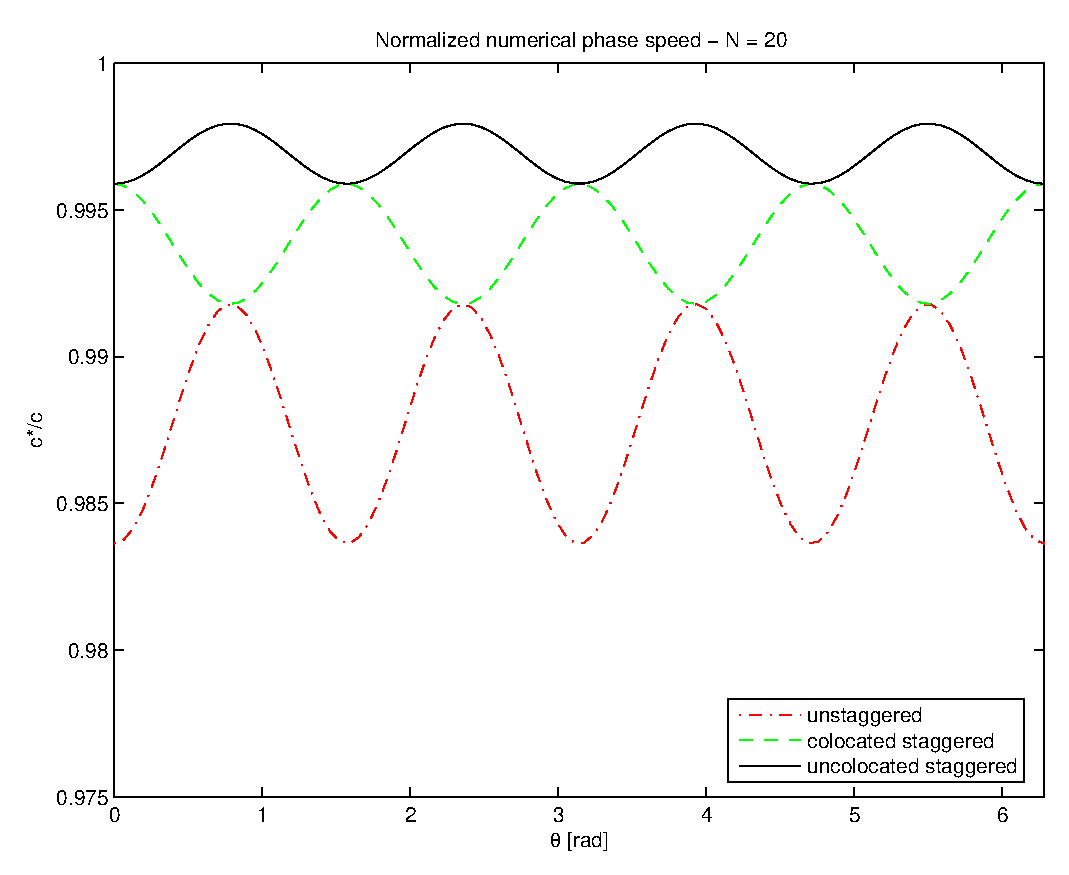
\includegraphics[height=8cm]{pics/liu_fourier_fig3}
  \end{center}
  \caption{Comparison of the normalized numerical phase speeds for
    Cartesian grids.}
  \label{fig:numerical_c}
\end{figure}  

From the \eqref{eqn:fourier_numerical_c2} we can note that the unstaggered
grid requires twice the number of points per wavelength in each
direction in order to have the same numerical phase speed as the
uncollocated staggered grid. In other words, for a given grid spacing
$\Delta s$, the error for the high frequency modes is greater than for
the low frequency modes, because we have less points per wavelength.

The error, defined as $1 - \frac{\Dual{c}}{c}$, is anisotropic
\eqref{fig:numerical_c_polar}: greatest along the axes ($\theta = 0,
\pi/2, \pi, 3\pi/2$) and least along the diagonals ($\theta = \pi/4,
3\pi/4, 5\pi/4, 7\pi/4$) for both the unstaggered and uncollocated
staggered grids. The opposite is true for the collocated staggered
grid. Note that, even if a proper choice of the discretization scheme
in time can improve the overall dispersive error, it cannot completely
cancel it. This error depends only on the spatial discretization: the
medium ``grid'' is anisotropic itself.

\begin{figure}[htbp]
  \begin{center}
    \subfigure[Unstaggered]{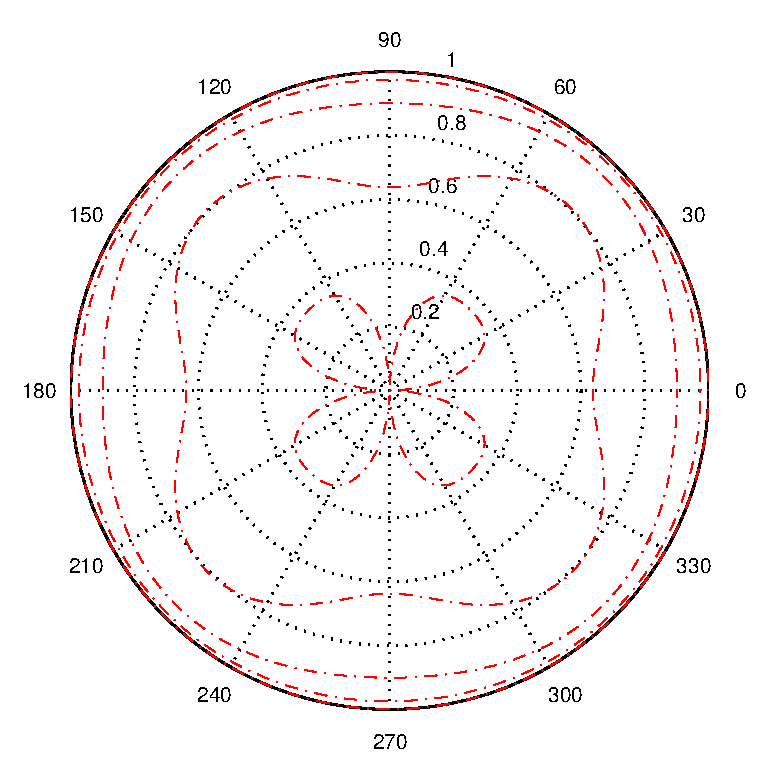
\includegraphics[width=3.5cm]{pics/liu_fourier_fig2a}}
    \subfigure[Collocated staggered]{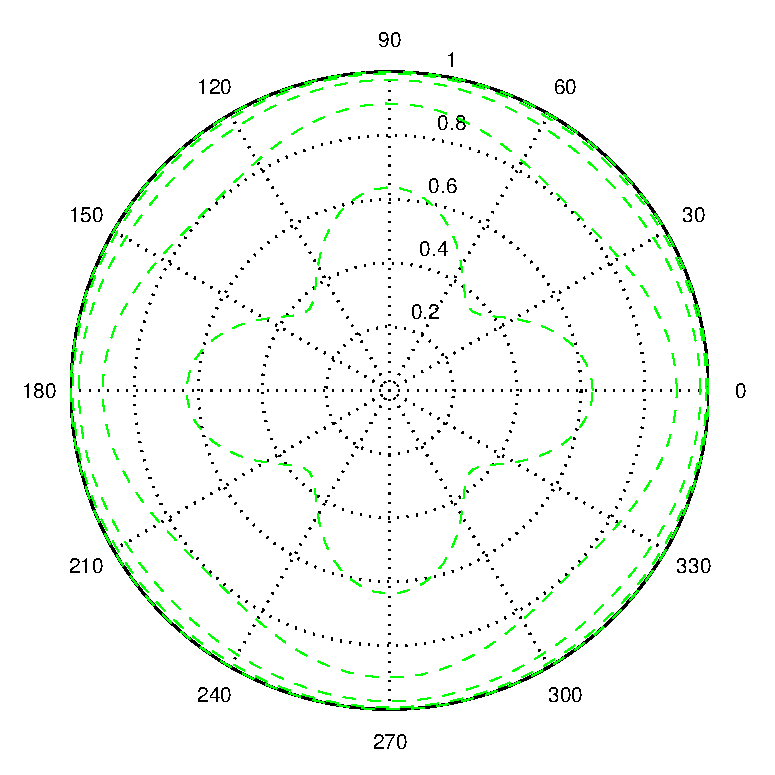
\includegraphics[width=3.5cm]{pics/liu_fourier_fig2b}}
    \subfigure[Uncollocated staggered]{\includegraphics[width=3.5cm]{pics/liu_fourier_fig2c}}
  \end{center}
  \caption{Polar diagrams of the normalized numerical phase speed for
    Cartesian grids and $N = 2, 4, 8, 16$.}
  \label{fig:numerical_c_polar}
\end{figure}  

We can define the \emph{isotropy error} as the difference between the
maximum and the minimum values of the normalized numerical phase speed
and we find that, for $N = 20$, it is $0.8\%$ on the unstaggered grid,
$0.4\%$ on the collocated staggered grid and $0.2\%$ on the uncollocated
staggered grid. In other words, to have the same isotropy error of
$0.1\%$ for the three schemes we need $N = 58, 41, 29$ grid points per
wavelength, respectively.

The dependence of the isotropy error on $N$ can be described expanding
in Taylor series the equations \eqref{eqn:fourier_numerical_c2}:
\begin{equation*}
  1-\frac{\Dual{c}}{c} = \begin{cases}
    \left( \frac{1}{2}  + \frac{1}{6} \cos 4\theta \right) \frac{\pi^2}{N^2} +
    \dotsb & \text{unstaggered} \\
    \left( \frac{1}{4}  - \frac{1}{12} \cos 4\theta \right) \frac{\pi^2}{N^2} +
    \dotsb & \text{collocated staggered} \\
    \left( \frac{1}{8}  + \frac{1}{24} \cos 4\theta \right) \frac{\pi^2}{N^2} +
    \dotsb & \text{uncollocated staggered} .
    \end{cases}
\end{equation*}

The leading dispersive errors are proportional to $N^{-2}$,
i.e. doubling the coarseness of the grid reduces the dispersive error
by a factor 4.

From these considerations it should be clear that the uncollocated
staggered grid is the best choice:
\begin{itemize}
\item
  it is more computationally efficient, as shown in \eqref{eqn:fourier_uncollocated_staggered};
\item
  it is 4 and 2 times more precise than the unstaggered and collocated
  staggered schemes, respectively, from a dispersive error point of
  view, as shown in \eqref{eqn:fourier_numerical_c2}.
\end{itemize}

\index{Cartesian grid|)}

\subsection{Hexagonal Grids} \index{Hexagonal grid|(}

The major deficiencies of conventional schemes come from their one
dimensional approach in which each spatial operator is approximated by
employing data only along one coordinate line. Since only a five point
Cartesian stencil is involved in each discretization, it is not
surprising that all three schemes described in the previous subsection
exhibit some anisotropy.

In this subsection we'll analyze a more efficient and accurate scheme,
not based on an orthogonal grid, but on a 7-point stencil on regular
hexagonal or triangular grid. This can also give a hint on the accuracy
of unstructured grids, which are topologically equivalent to this one.

We also use the information of the previous subsection, in which we
concluded that the uncollocated staggered scheme is the most efficient,
and we'll limit our study to the same scheme, but applied to the new
triangular grid.

\figref{fig:liu_fig4} shows two possible hexagonal discretization schemes:
unstaggered or staggered. We will focus our attention only on the
staggered one, which is the topological equivalent of the
discretization scheme described in \charef{cha:discretization_schemes}.

\begin{figure}[htbp]
  \begin{center}
    \subfigure[Unstaggered.]{\resizebox{3.5cm}{!}{\input{pics/liu_fig4a.pdf_t}}}
    \subfigure[Staggered.]{\label{fig:liu_fig4b}\resizebox{3.5cm}{!}{\input{pics/liu_fig4b.pdf_t}}}
  \end{center}
  \caption{Placement of unknowns on two-dimensional hexagonal grids.}
  \label{fig:liu_fig4}
\end{figure}

With respect to \figref{fig:liu_fig4b}, \eqref{eqn:fourier_maxwell_2d}
can be discretized as follows:
\begin{equation} \label{eqn:fourier_hexagonal_grid} \begin{split}
    d_t \Disc{D_z}{j,k}{} & = \frac{2 \left( \begin{aligned}
	\Disc{H_1}{j+1/4,k-\sqrt{3}/4}{} & -
	\Disc{H_1}{j-1/4,k+\sqrt{3}/4}{} + \\
	\Disc{H_2}{j+1/2,k}{} & - \Disc{H_2}{j-1/2,k}{} + \\
	\Disc{H_3}{j+1/4,k+\sqrt{3}/4}{} & -
	\Disc{H_3}{j-1/4,k-\sqrt{3}/4}{}
    \end{aligned} \right)}{3 \Delta s} \\
    d_t \Disc{B_1}{j+1/4,k-\sqrt{3}/4}{} & =
    \frac{\Disc{E_z}{j+1/2,k-\sqrt{3}/2}{} - \Disc{E_z}{j,k}{}}{\Delta s} \\
    d_t \Disc{B_2}{j+1/2,k}{} & = \frac{\Disc{E_z}{j+1,k}{} -
    \Disc{E_z}{j,k}{}}{\Delta s} \\
    d_t \Disc{B_3}{j+1/4,k+\sqrt{3}/4}{} & =
    \frac{\Disc{E_z}{j+1/2,k+\sqrt{3}/2}{} - \Disc{E_z}{j,k}{}}{\Delta s} .
\end{split} \end{equation}

Again, the eigenvalues of the corresponding matrix $\Matrix{G}_s$ are
pure imaginary or zero, implying that this scheme is non-dissipative,
but dispersive.

Applying the Fourier analysis to the above equations, we obtain the
normalized numerical phase speed:
\begin{equation}
  \frac{\Dual{c}}{c} = \frac{\sqrt{8/3}}{\kappa \Delta s}\left[
  \sin^2 \frac{\xi}{2} + \sin^2 \left(\frac{\xi}{4} -
  \frac{\sqrt{3}\eta}{4}\right) + \sin^2 \left(\frac{\xi}{4} +
  \frac{\sqrt{3}\eta}{4}\right)\right]^{1/2}
\end{equation}
and the isotropy error:
\begin{equation}
  1-\frac{\Dual{c}}{c} = \frac{1}{8}\frac{\pi^2}{N^2} -
  \left(\frac{7}{1152} + \frac{1}{720} \cos 6\theta\right) \frac{\pi^4}{N^4} +
  \dotsb .
\end{equation}

\begin{figure}[htbp]
  \begin{center}
    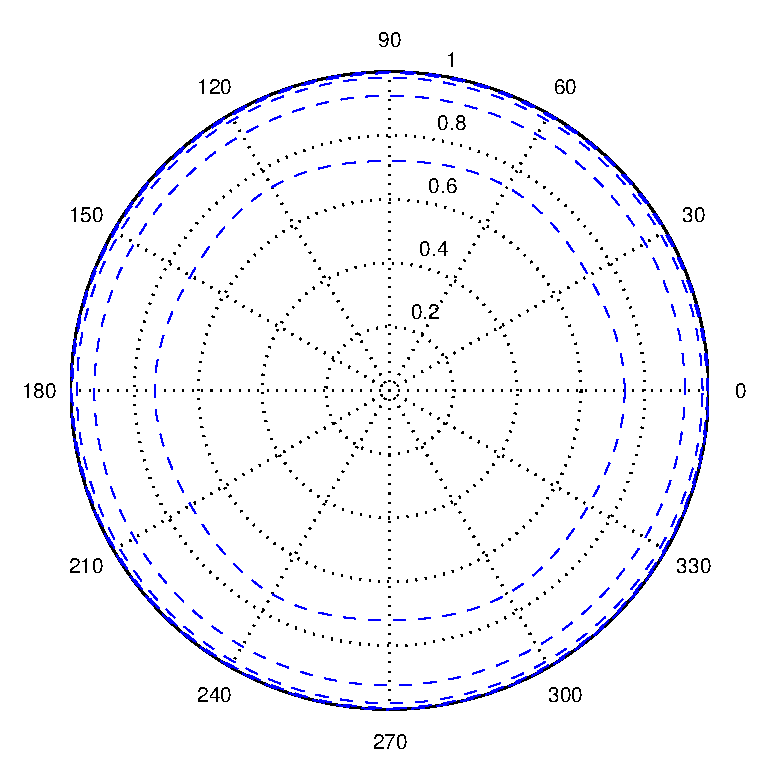
\includegraphics[height=8cm]{pics/liu_fourier_fig5b}
  \end{center}
  \caption{Polar diagram of the normalized numerical phase speed for
    hexagonal grids.}
  \label{fig:numerical_c_polar_hex}
\end{figure}  

\begin{figure}[htbp]
  \begin{center}
    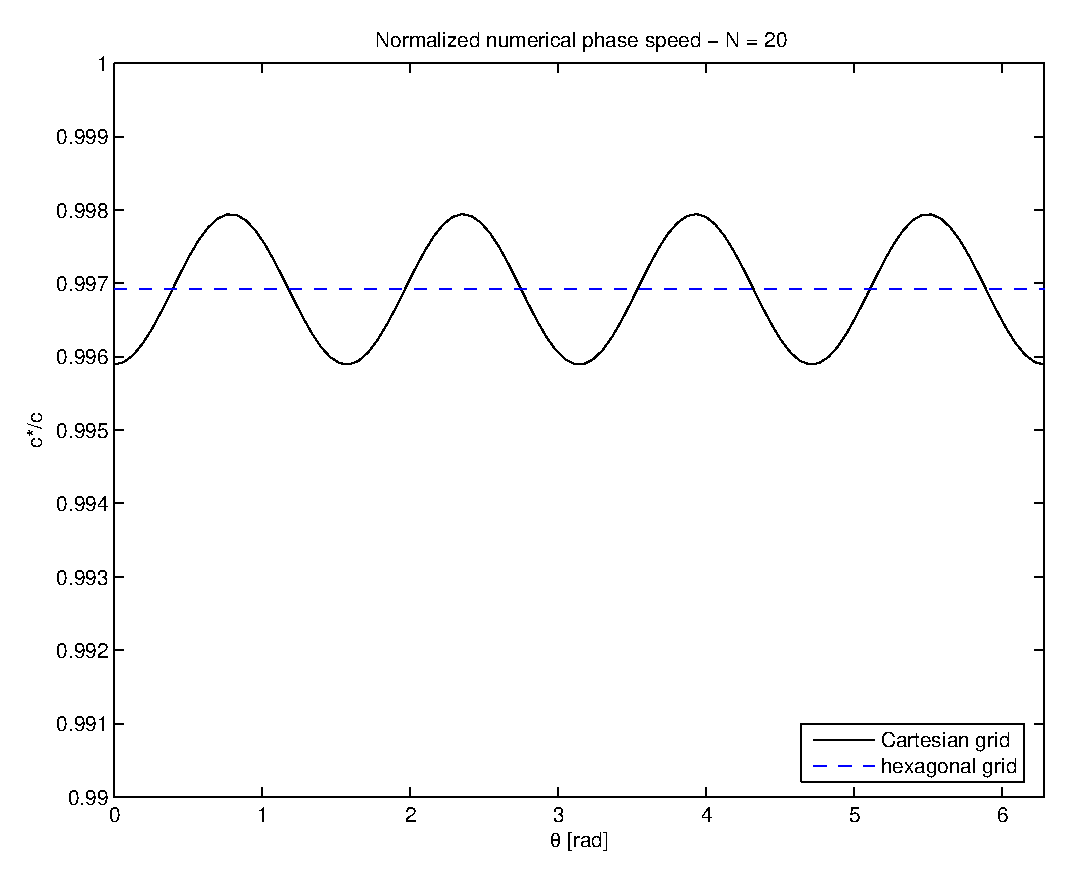
\includegraphics[height=8cm]{pics/liu_fourier_fig6}
  \end{center}
  \caption{Comparison of the normalized numerical phase speed for
    uncollocated staggered grids: Cartesian and hexagonal.}
  \label{fig:numerical_c_hex}
\end{figure}  

Even if the isotropy error is still leaded by a term proportional to
$N^{-2}$, \figref{fig:numerical_c_polar_hex} shows that it doesn't
depend anymore on the direction of the wave propagation. Quite
surprisingly, its value is exactly the average of its Cartesian
counterpart, as shown in \figref{fig:numerical_c_hex}.

The anisotropy appears in the fourth order term, which is two orders
of magnitude smaller than in the best Cartesian grid.

From these results, we conclude that uncollocated staggered hexagonal
grids are clearly superior to Cartesian grids from a numerical error
point of view: Cartesian grids require less operations and, if
implemented on a computer, lead to a faster algorithm. A complete
analysis of unstructured grids is prohibitive, because an
analytical expression for the isotropy error is not possible: for each
possible unstructured grids, an eigenvalue problem should be solved,
to extract its characteristics. Being topologically equivalent to
hexagonal grids, though, we can expect them to present the same good
numerical errors characteristics. Moreover, they permit to discretize
some parts of the computational domain with a coarser grid: this is a
clear advantage over both Cartesian and hexagonal grids, whose
gridspacing is constant everywhere. This becomes a speed advantage in
a computer implementation.

\index{Hexagonal grid|)}
\index{Stability!space discretization|)}
\index{Discretization schemes|)} 








%% \section{Structured}
%% \begin{itemize}
%% \item
%%   easy to build
%% \item
%%   easy to manage
%% \item
%%   staircase approximation \cite{cangellaris_analysis}
%% \item
%%   anisotropy of the medium ``grid'' \cite{liu_fourier}
%% \end{itemize}

%% \subsection{Orthogonal}
%% diagonal constitutive matrices: local relations, stable

%% \subsection{Non-Orthogonal}
%% non diagonal constitutive matrices: non local constitutive relations,
%% more unstable (depending on the minimum angle). Mainly used in
%% association with periodic boundary conditions to simulate non
%% orthogonal primitive cells in periodic structures.




%% \section{Unstructured}
%% Numerical Errors of the Stair-Cased approximation
%% \cite{cangellaris_analysis}

%% \begin{itemize}
%% \item
%%   better discretization of the domain (tangential fields always
%%   continuous)
%% \item
%%   less memory: coarser grid where I don't need it
%% \item
%%   more difficult to generate and manage (meshing software survey)
%% \end{itemize}

%% Unstructured grids in 3D are difficult: 2.5D! unstructured in 2D,
%% structured in the third dimension: layered structured
%% \cite{gedney_parallel}.

%% Triangles as simplicials is the most general choice. How do I choose
%% the dual grid?

%% \subsection{Delaunay-Vorono\"{i}} \label{sec:delaunay_voronoi}
%% properties and difficulty in generating it (direct analogous to the
%% orthogonal structured grid, but unstructured): local constitutive
%% relations

%% \subsection{Poincar\'e}
%% easier to build, but non local relations (non diagonal stiffness matrix)

%% \subsection{Barycentric}
%% the more general and stable scheme, but much more complex to implement
%% (ref. marrone, tonti, bossavit)




%% \section{Structured vs. Unstructured aka Refractive Index Smoothing}


%% \section{Blah Blah}

%% from the Maxwell's equations to a matricial formulation
%% \begin{itemize}
%% \item
%%   mapping of geometrical entities with physical quantities
%%   \cite[pag. 40]{bossavit_computational}: constituive laws are
%%   mappings between p-forms and (3-p)-forms.
%% \item
%%   Primary and dual grid: Maxwell's paper on the geometrical
%%   association of physical quantities \cite{maxwell_mathematical}: all
%%   on the primary grid leads to numerical losses (non physical)
%% \item
%%   Maxwell's equations are topological relations about geometrical
%%   quantities: what makes different schemes different are the
%%   ``Constitutive relations'' --> Tonti
%% \item
%%   Stability problem: Maxwell's equation as a ``control problem'': all
%%   the eigvals must lie in precise positions --> Taflove
%% \end{itemize}

%% for each scheme: constitutive laws, pros, cons.

%% \OKKIO{meshing softwave!}

%% \OKKIO{pag. 107 - equazioni di maxwell in formulazione
%%   integrale/globale}

%% \OKKIO{pag. 144 - interpolazione dei valori dentro al un simplesso
%%   (coordinate baricentriche)}

%% \OKKIO{vettori assiali (B,H,M) e polari (E,P,E,J,S) - appendice A}

%% \OKKIO{covarianza e controvarianza: appendice C}


%% \OKKIO{From \cite{rienen_frequency}.}

%% \begin{definition}[dual grid]
%%   A dual grid $\Dual{G}$ is defined as:
%%   \begin{itemize}
%%   \item
%%     $\Dual{G}$ as $G$, with $\Dual{V}$, $\Dual{A}$, $\Dual{L}$ and
%%     $\Dual{P}$;
%%   \item
%%     $\forall \Dual{V}_j \, \exists P_i$ with $P_i \in \Dual{V}_j$, $\forall
%%     V_j \, \exists \Dual{P}_i$ with $\Dual{P}_i \in V_j$;
%%   \item
%%     $\forall \Dual{A}_j \, \exists L_i$ with $L_i \bigcap \Dual{A}_j \neq
%%     \EmptySet$, $\forall A_j \, \exists \Dual{L}_i$ with $\Dual{L}_i
%%     \bigcap A_j \neq \EmptySet$.
%%   \end{itemize}
%% \end{definition}

%% \OKKIO{orientazione della mesh duale discende da quella della mesh
%%   primale: interna diventa esterna e viceversa}

%% \OKKIO{elementi temporali: istanti e intervalli; orientazione: istanti
%%   primali -> pozzi (come i punti spaziali -- definizione di derivata nel
%%   tempo), intervalli primali -> orientazione interna nel senso degli
%%   istanti crescenti. elementi del complesso duale subiscono
%%   l'orientazione dei corrispondenti elementi primali: istanti duali ->
%%   orientazione esterna (come gli intervalli primali), intervalli duali
%%   -> orientazione esterna (come gli istanti primali). Inversione
%%   temporale: grandezze associate a istanti duali (carica elettrica che
%%   fluisce) o intervalli primali cambiano segno per inversione temporale
%%   (cioe' se inverto l'orientazione interna degli intervalli primali),
%%   quelli associati agli intervalli duali (carica elettrica contenuta) o
%%   agli istanti primali no}

%%  The two complexes form the
%% mesh $\Set{M} = \left\{ \Set{K}, \Dual{\Set{K}} \right\}$.

%% $\Array{m}$ is the
%% magnetic charge density and $\Array{\rho}_e$ ($\Array{\rho}_m$) is the
%% electric (magnetic) charge density\footnote{No magnetic monopole is
%% known in Nature by now, but it's somehow reassuring that the formalism
%% of Maxwell's equations wouldn't fail if it existed.}

%%   \Array{\rho}_m & \in \CrossProd{\nv}{1} & \Array{\rho}_e & \in \CrossProd{\ndv}{1}
